%&pdflatex
%
%  Guerrero Gap Earthquake/Tsunami Model
%
%  Created by Kyle T. Mandli and Hugo Cruz
%  Copyright (c) 2014 University of Texas at Austin. All rights reserved.
%  Copyright (c) 2014 KAUST.  All rights reserved
%
% \documentclass[preprint,12pt]{elsarticle}
%% Use the option review to obtain double line spacing
\documentclass[preprint,review,12pt]{elsarticle}

% Use utf-8 encoding for foreign characters
\usepackage[utf8]{inputenc}

% Setup for fullpage use
\usepackage{fullpage}

% Uncomment some of the following if you use the features
%
% Running Headers and footers
%\usepackage{fancyhdr}

% Multipart figures
% \usepackage{caption}
\usepackage{subcaption}

\synctex=1

% More symbols
\usepackage{amsmath}
\usepackage{amssymb}
\usepackage{latexsym}

% URL and linking help
\usepackage{hyperref}

% Surround parts of graphics with box
% \usepackage{boxedminipage}

% Package for including code in the document
\usepackage{listings}

% This is now the recommended way for checking for PDFLaTeX:
\usepackage{ifpdf}

% Add line numbers
\usepackage[mathlines]{lineno}

% Commands
% Need to use this package to handle the spacing issues in LaTeX after a command
\usepackage{xspace}
\newcommand{\geoclaw}{{\sc GeoClaw}\xspace}
\newcommand{\compsyn}{COMPSYN\xspace}
\newcommand{\pd}[2]{\ensuremath{\frac{\partial #1}{\partial #2}}} % partial

% Graphics
% \DeclareGraphicsRule{.tif}{png}{.png}{`convert #1 `dirname #1`/`basename #1 .tif`.png}
\graphicspath{{./figures/}}
% \usepackage{epstopdf}

\usepackage{color}
\newcommand{\alert}[1]{\textbf{\color{red} #1}}

% \journal{}

\begin{document}

\ifpdf
\DeclareGraphicsExtensions{.pdf, .png, .jpg, .tif}
\else
\DeclareGraphicsExtensions{.png, .jpg, .tif, .eps}
\fi

\begin{frontmatter}

\title{Inundation maps in Acapulco Bay, Mexico due to a tsunami triggered by a Mw 8.2 earthquake in the Guerrero Gap}

\author[kaust1]{Hugo Cruz\corref{cor1}}
\author[ut]{Kyle T. Mandli}
\author[kaust1,kaust2]{Ibrahim Hoteit}
\author[ut]{Clint N. Dawson}

\ead{Hugo.CruzJimenez@kaust.edu.sa}
\cortext[cor1]{Corresponding author}

\date{\today}
\address[kaust1]{Division of Physical Sciences and Engineering, King Abdullah University of Science and Technology, Thuwal, Saudi Arabia}
\address[ut]{Institute for Computational Engineering and Science, University of Texas at Austin, 201 E 24th ST. Stop C0200, Austin, TX 78712-1229, USA}
\address[kaust2]{Division of Computer, Electrical and Mathematical Sciences and Engineering, King Abdullah University of Science and Technology, Thuwal, Saudi Arabia}

\date{\today}

\begin{abstract}

\end{abstract}

\begin{keyword}
tsunami \sep Guerrero Gap \sep fault mechanisms
\end{keyword}

\end{frontmatter}
\linenumbers


\section{Abstract}

\begin{itemize}
  \item Here we mention that the Acapulco Bay and other coastal areas along the Mexican Pacific coast could be affected by a big tsunami in case a Mw 8.2 earthquake occurs in the Guerrero Gap (Mexico). 
  \item The necessity of having inundation maps in Acapulco, an important tourist resort, in order to develop evacuation plans to reduce damages and lose of lives. 
  \item We mention our approach and that we perform a sensitivity analysis considering changes in the earthquake rupture model. 
  \item We finalize it with key results of our simulations.
\end{itemize}

\section{Introduction} \label{sec:intro}

\begin{itemize}
  \item Here we present a narrative of some of the most significant tsunamis (and their great damages) occurred  in the last century (e.g. those triggered by the Chile, 1960 and Alaska, 1964 earthquakes) and last decade  (Indonesia, 2004 and Japan, 2011) around the world.
   \item Some examples of subduction zones where other tsunamis could occur and the areas they could affect.
  \item We point out the necessity of having inundation maps and preparing emergency/evacuation plans at coastal areas that could be seriously affected by tsunamis.
  \item Brief description of previous tsunamis observed in and at the neighbourhood of the Acapulco Bay.
  \item Here clearly we point out that the Acapulco Bay is threatened by a big tsunami that could be triggered by a Mw 8.2 earthquake in the Guerrero Gap.
  \item Previous studies of past tsunamis such as the ones triggered by the San Marcos, 1957 and Michoacan, 1985 earthquakes.
  \item A description of some studies that consider instantaneous (Okada's approach) or time-dependent sea floor deformation. 
  \item We mention that our approach incorporates time-dependent sea floor deformation with geoclaw.
  \item Finally, we mention that we present a sensitivity study considering several configurations which include: 2 different fault locations with respect to the trench, rupture speeds, epicenter location along the fault plane and depth of the hypocenter.
\end{itemize}

       
\section{Tectonic framework and seismicity in the Guerrero Seismic Gap} \label{sec:tectonic_guerrero_gap}
\emph{Maybe this could be in the intro as a review of our understanding of the area?}

\begin{itemize}
  \item A description of the tectonic framework of the area.
  \item A general description of the seismicity along the Mexican Subduction Zone.
  \item A detailed description of the seismicity of the area indicating the largest events occurred about 100 years ago (with the hypothesis of the expected Mw 8.2 earthquake in the gap), as well as the recent activity of March and April, 2014 in Petatlan, Guerrero.
\end{itemize}

\section{Data} \label{sec:data}

A detailed description of the resolution of the data we use in our study, including their sources (organizations).
\begin{itemize}
  \item Topography
  \begin{itemize}
    \item SRTM
    \item GEBCO data
    \item Private source
  \end{itemize}
  \item Bathymetry
  \begin{itemize}
    \item GEBCO
    \item Private source
  \end{itemize}
  \item Tide gauge recordings
\end{itemize}

\section{Method} \label{sec:method}

\subsection{\compsyn} \label{sub:compsyn}
\emph{A description about \compsyn and configuration of seismic stations around the fault plane (shown in a clear figure) where we obtain the displacement.}

\subsection{\geoclaw} \label{sub:geoclaw}

\emph{A description about GeoClaw, the incorporation of sea-floor deformation, topography and bathymetry, and how AMR works.}

We utilized the \geoclaw package for performing all forward model runs.  \geoclaw uses a finite volume, wave-propagation approach to solve the two-dimensional nonlinear shallow water equations
\begin{equation} \label{eq:swe}
    \begin{aligned}
    &\pd{}{t} h + \pd{}{x} (hu) + \pd{}{y} (hv) = 0, \\
    &\pd{}{t}(hu) + \pd{}{x} \left(hu^2 + \frac{1}{2} g h^2 \right ) + \pd{}{y} (huv) = ~~ fhv - gh \pd{}{x} b - C_f |\vec{u}| hu \\
    &\pd{}{t} (hv) + \pd{}{x} (huv) + \pd{}{y} \left (hv^2 + \frac{1}{2} gh^2 \right) = -fhu - gh \pd{}{y} b - C_f |\vec{u}| hv
    \end{aligned}
\end{equation}
where $h$ is the depth of the water column, $u$ and $v$ the velocities in the longitudinal and latitudinal directions respectively, $g$ the acceleration due to gravity, $b$ the bathymetry, $f$ the Coriolis parameter, and $C_f$ the bottom friction coefficient determined by a Manning's $n$ parameterization such that
\begin{equation}
    C_f = \frac{g n^2}{h^{5/3}}
\end{equation}
where $n$ is an empirically determined parameter.

The primary computational kernel in \geoclaw is the evaluation of the solution to the Riemann problem at each grid cell interface.  The Riemann solver used includes the ability to handle inundation (wet-dry interfaces), well-balancing even when the momentum is non-zero, and entropy corrections \cite{George:2008aa}.

\emph{Need to add discussion of AMR here}

\subsubsection{Fault Movement Handling} \label{ssub:fault_movement}

Fault movement in \geoclaw is handled differently depending on the type of movement specified.  At its simplest, a single deformation from the original bathymetry is specified and at the beginning of the simulation the bathymetry and therefore the surface is deformed accordingly (see Figure~\ref{fig:fault_movement_diagram}).  If the fault is specified with a temporal displacement, then a series of snapshots of the deformation are read in and the topography modified at the specified times.  In the case of the deformations presented, a final deformation was taken and linearly interpolated from $t=0$ to the end time at $5$ second intervals.

% \begin{figure}[tb]
%     \begin{center}
%         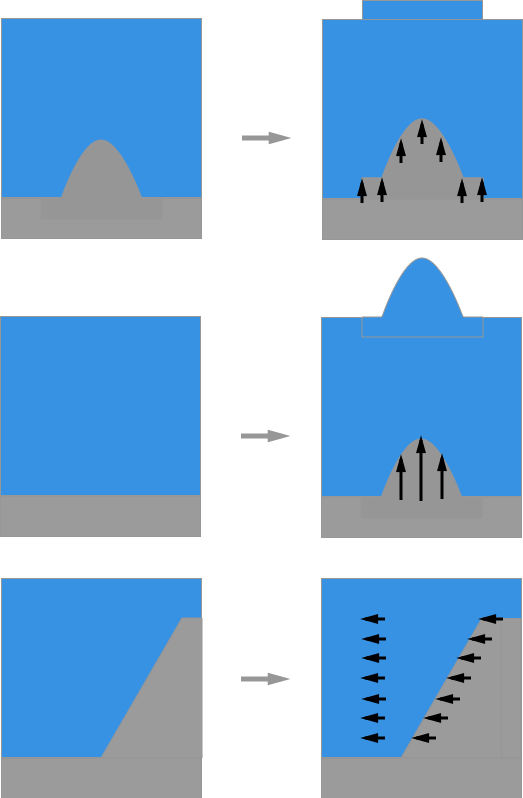
\includegraphics[width=0.8\textwidth]{earth_quake_tsunami_source.png}
%     \end{center}
%     \caption{Caption here}
%     \label{fig:fault_movement_diagram}
% \end{figure}

\subsection{Okada Model} \label{sub:okada}

\emph{A small description about pros and cons of Okada's model.}

\section{Validation of our approach} \label{sec:validation}
\emph{Maybe change this to a subsection?}
\begin{itemize}
  \item In this section we consider the small tsunami (50 cm high) of the Petatlan earthquake (Mw 7.2; March 2014). 
  \item We use instantaneous displacement (Okada's approach) given its relatively small fault length (55 km).
  \item We use fault planes located around the aftershock distribution.
  \item We show the fitting between simulated tsunami waveforms with the observed tide gauge recording at Acapulco.
\end{itemize}

\section{Rupture models and sea-floor deformations} \label{sec:rupture_models}

In this section we describe all rupture models and corresponding sea floor deformations for the Mw 8.2 earthquake. We begin with a simple deformations given by Okada's approach and then with those from the time-dependent approach. We show some figures indicating areas of the largest deformations which will help us to explain differences in inundation maps.

\begin{enumerate}
  \item Instantaneous sea floor deformation obtained with Okada's approach.
%  \item Displacement distribution with stochastic slip distributions with higher amplitudes near the surface, considering 
  \item Time-dependent sea floor deformation obtained from a rupture model that considers a shallow fault plane (closer to the trench), with top of the fault at 1 km depth, hypocenter at a depth of 3.5 km, different epicenter location along the fault plane and different rupture speed, as shown below:

  \begin{enumerate}
    \item Epicenter at the Southeastern edge of the fault plane
    \begin{itemize}
      \item Rupture speed= 1.0 km/s 
      \item Rupture speed= 2.0 km/s 
      \item Rupture speed= 2.7 km/s 
    \end{itemize}

    \item Epicenter at the center of the fault plane
    \begin{itemize}
      \item Rupture speed= 1.0 km/s 
      \item Rupture speed= 2.0 km/s 
      \item Rupture speed= 2.7 km/s 
    \end{itemize}

    \item Epicenter at the Northwestern edge of the fault plane
    \begin{itemize}
      \item Rupture speed= 1.0 km/s 
      \item Rupture speed= 2.0 km/s 
      \item Rupture speed= 2.7 km/s 
    \end{itemize}
\end{enumerate}

  \item Time-dependent sea floor deformations similar to the previous ones but with a deeper fault plane (farther from the trench), with top of the fault at 5 km depth, and hypocenter at a depth of 7 km.

  \begin{enumerate}
   \item Same epicenters and rupture speeds as above.
  \end{enumerate}

   \item If necessary, another set of simulations with a fault plane even deeper and farther from the trench (with a significant part inshore). 

  \item Alternatively, given that I got topography that includes infrastructure (hotels, houses, etc ...), we could incorporate more simulations (as those in 2 and 3) and compare them.
\end{enumerate}

\section{Tsunami simulations of the hypothetical Mw 8.2 earthquake in the Guerrero Gap} \label{sec:guerrero_gap}
\begin{itemize}
  \item Here we simulate tsunamis considering deformations mentioned above corresponding to the  hypothetical Mw 8.2 earthquake in the Guerrero Gap. 
  \item We show inundation maps as well as run-up heights for each case.
\end{itemize}

\section{Sensitivity analysis} \label{sec:sensitivity}

\begin{itemize}
  \item  In this section we analyze all inundation maps and run-up heights produced by the different sea floor deformations and explain differences in terms of rupture speed, hypocenter and location of the fault plane with respect to the trench. 
 \item We highlight the areas with largest inundation along the bay.
\end{itemize}

\section{Discussion} \label{sec:discussion}

\begin{itemize}
  \item We discuss about our results, how they change depending on the involved parameters(depth of the top of the fault, hypocenter, rupture speed).
  \item We show the areas along the Acapulco bay that could be seriously affected, and how our results could help to prepare emergency plans to reduce damages. 
  \item We definitely have to mention about the limitations of our approach. 

  \begin{enumerate}
   \item \compsyn fails for cases when the fault ruptures  the surface. We have to mention the necessity to conduct more realistic simulations (including dynamic ones) which consider rupture of the sea floor surface and their implications on the inundation maps. 
   \item We could consider other slip distributions (asperities) on the fault plane and check how they could affect the sea floor deformation.
   \item GeoClaw does not include a dispersive term, which could change significantly our results, specially near the source area.
   \item We can mention that our simulations consider a Manning friction coefficient of 0.025, but that inundation extension would change if we use different values.
  \end{enumerate}

\end{itemize}
  
\section{Conclusions} \label{sec:conclusions}

\begin{itemize}
\item Here we give a general description of our results highlighting mainly the areas that could be affected seriously. 
  \item We point out the necessity of future studies such as dynamic simulations of the rupture process and rupture of the sea-floor surface.
\end{itemize}

% ==============================================================================
%  Acknowledgments
\vskip 10pt
{\bf Acknowledgments.}


\bibliographystyle{plain}
\bibliography{database}

\end{document}